% !TEX program = pdflatex
% PyISIS IEEE JSTARS Paper - IMRaD Format with Style Transfer
% Converted: 2026-05-31
% Based on IEEE Transactions LaTeX template
%
% Compile with:
%   pdflatex paper_pyisis_jstars_imrad.tex
%   bibtex paper_pyisis_jstars_imrad
%   pdflatex paper_pyisis_jstars_imrad.tex
%   pdflatex paper_pyisis_jstars_imrad.tex

\documentclass[lettersize,journal]{IEEEtran}

% Core packages (IEEE JSTARS standard)
\usepackage{amsmath,amsfonts}
\usepackage{algorithmic}
\usepackage{algorithm}
\usepackage{array}
\usepackage[caption=false,font=normalsize,labelfont=sf,textfont=sf]{subfig}
\usepackage{textcomp}
\usepackage{stfloats}
\usepackage{url}
\usepackage{verbatim}
\usepackage{graphicx}
\usepackage{cite}
\usepackage{booktabs}
\usepackage{multirow}
\usepackage{tabularx}
\usepackage{hyperref}

% Figure paths
\graphicspath{{figures/}}

% Custom commands
\newcommand{\pyisis}{PyISIS}
\newcommand{\isis}{ISIS}
\newcommand{\sift}{SIFT}
\newcommand{\flann}{FLANN}

\hyphenation{op-tical net-works semi-conduc-tor IEEE-Xplore}

\begin{document}

\title{PyISIS: A Python-Bridged Planetary Photogrammetry Framework with Adaptive Deep Learning Image Matching for Automated Control Network Construction}

\author{Xun~Geng%
\thanks{This work was supported by the National Natural Science Foundation of China under Grant XXXXXXXX. (Corresponding author: Xun Geng.)}%
\thanks{The author is with the School of Geography and Tourism, Henan University, Kaifeng 475004, China (e-mail: gengxun@henu.edu.cn).}
}

% The paper headers
\markboth{IEEE Journal of Selected Topics in Applied Earth Observations and Remote Sensing, Vol.~XX, No.~XX, Month~2026}%
{Geng \MakeLowercase{\textit{\huge:}} PyISIS Framework for Planetary Photogrammetry}

\IEEEpubid{XXXX-XXXX/XX\$00.00~\copyright~2026 IEEE}

\maketitle

\begin{abstract}
The USGS Integrated Software for Imagers and Spectrometers (ISIS) remains a core platform for planetary image processing, but its C++ application interface makes it difficult to combine rigorous camera geometry with modern Python-based image matching workflows. This paper presents \pyisis{}, a pybind11-based Python binding framework that exposes ISIS 9.0.0 camera models, SPICE navigation kernels, map projections, photometric models, and control-network classes to Python. Building on this binding layer, we develop a control-network construction workflow that combines classical SIFT matching, learned sparse matching, detector-free matching, and an adaptive routing layer. The routing layer does not claim a new feature matcher. Instead, it uses texture diagnostics, SPICE-derived solar geometry, and post-match quality gates to decide when a low-cost classical matcher is sufficient and when escalation to LightGlue or LoFTR is warranted. Experiments on Lunar Reconnaissance Orbiter (LRO) Narrow Angle Camera (NAC) imagery show that the workflow can generate ISIS-compatible control networks while preserving C++ numerical behavior for camera coordinate transformation, solar-geometry evaluation, and ControlNet traversal. We further frame ISIS \texttt{findfeatures} as the domain-standard feature-based control-network baseline and define a controlled comparison protocol against fixed SIFT, LightGlue, LoFTR, and adaptive routing. The results support the value of SPICE-aware matcher orchestration for heterogeneous lunar polar imagery, while also identifying the need for expanded \texttt{findfeatures} and bundle-adjustment validation before making mission-scale accuracy claims.
\end{abstract}

\begin{IEEEkeywords}
planetary photogrammetry, image matching, deep learning, control network, feature detection, adaptive routing, ISIS, pybind11, lunar remote sensing
\end{IEEEkeywords}

% ============================================================================
% I. INTRODUCTION
% ============================================================================

\section{Introduction}
\IEEEPARstart{C}{ontrol} network construction is a fundamental task in planetary photogrammetry, enabling precise geometric relationships between overlapping images for map production, topographic modeling, and mission navigation \cite{archinal2018iau,robinson2010lroc}. Planetary exploration missions generate vast quantities of imaging data that require precise geometric processing for scientific analysis and mission operations. Control networks—collections of tie points measured across overlapping images—form the geometric backbone of planetary cartography, enabling bundle adjustment, digital terrain model (DTM) generation, and image mosaic production. The construction of high-quality control networks remains one of the most labor-intensive tasks in planetary photogrammetry, particularly for large mapping campaigns involving hundreds or thousands of images. Indeed, the difficulty of constructing reliable control networks increases substantially when images are acquired under varying illumination conditions or over terrain with sparse surface texture, both of which are common in planetary remote sensing.

The USGS Integrated Software for Imagers and Spectrometers (ISIS) has been the cornerstone of planetary image processing since its inception in the 1990s, supporting over 50 planetary missions spanning the Moon, Mars, Mercury, Venus, the outer planets, and small bodies \cite{usgs2024isis}. ISIS provides comprehensive capabilities for radiometric calibration, geometric processing, photogrammetric control, and map projection through a suite of command-line applications such as \texttt{lronaccal}, \texttt{spiceinit}, \texttt{cam2map}, and \texttt{jigsaw}. However, its C++ architecture and application-centric design present fundamental limitations for modern research workflows. Contemporary photogrammetric research increasingly adopts Python for scientific computing, leveraging ecosystems such as NumPy, SciPy, OpenCV, PyTorch, and Kornia. Direct integration of ISIS functionality within Python workflows has been impractical, forcing researchers into fragmented pipelines that shuttle data between ISIS command-line tools and Python analysis scripts via intermediate file formats. The overhead associated with subprocess invocation and file I/O considerably degrades processing efficiency, particularly when iterative algorithm development is involved.

In recent years, the emergence of deep learning-based image matching methods has introduced new opportunities and challenges for planetary photogrammetry. Graph neural network matchers such as SuperGlue \cite{sarlin2020superglue} and LightGlue \cite{lindenberger2023lightglue}, and detector-free methods such as LoFTR \cite{sun2021loftr}, have demonstrated substantial improvements in matching robustness under challenging conditions including large illumination changes and sparse texture. Integrating these methods into ISIS-based workflows, however, requires complex middleware that bridges the gap between the C++ photogrammetric environment and Python-based deep learning libraries. Moreover, no single matching algorithm performs optimally across the full range of planetary imaging conditions. Classical methods such as SIFT \cite{lowe2004sift} excel on texture-rich imagery with similar illumination, while deep learning methods demonstrate superior performance under large illumination changes or on texture-poor surfaces. Manual selection of matching strategies requires expert knowledge and is impractical for large-scale processing campaigns. Recent benchmarking on 496 WorldView-3 stereo pairs with LiDAR ground truth \cite{satellite2024benchmark} provides strong empirical validation for multi-method approaches: no single method succeeded universally across diverse conditions, motivating cascade fallback designs. Therefore, there is a pressing need for an integrated framework that provides native Python access to ISIS geometric primitives while supporting adaptive selection among multiple matching strategies.

In this study, we propose a comprehensive pybind11-based Python binding framework named \pyisis{}, which exposes over 200 ISIS 9.0.0 C++ classes to Python, including camera models for 50+ planetary missions, Spacecraft, Planet, Instrument, Camera-matrix, and Events (SPICE) navigation kernels, control network manipulation, bundle adjustment, and photometric models. Building upon \pyisis{}, an integrated image matching and control network construction pipeline is developed that fuses classical descriptor-based methods with state-of-the-art deep learning matchers. The main contributions of our work are as follows:

1) We present the most comprehensive Python binding framework for USGS ISIS to date, exposing over 200 C++ classes and types via pybind11—covering camera models, SPICE navigation, control networks, bundle adjustment, projections, photometry, and shape models. The framework enables seamless integration of ISIS photogrammetric capabilities within Python scientific computing workflows, eliminating the subprocess overhead and file-based coupling of prior approaches.

2) We develop an integrated image matching pipeline that unifies classical (SIFT-BF, SIFT-FLANN) and deep learning (SuperGlue, LightGlue, LoFTR) matchers within a tile-based processing framework, together with an adaptive routing system that selects or cascades matchers according to quantitative image analysis. The system computes texture sparseness via tile-level SIFT density, gradient magnitude, and GLCM contrast, and lighting differences from SPICE-derived solar elevation and azimuth geometry. A cascade fallback mechanism (SIFT $\rightarrow$ LightGlue $\rightarrow$ LoFTR) progressively escalates to more capable methods when quality thresholds are not met. The contribution is a SPICE-aware orchestration layer for planetary control-network construction, not a replacement for existing feature matchers.

3) We present an end-to-end control network construction workflow that integrates \pyisis{} geometry, adaptive matching, and coordinate transformation from projected DOM space back to original image coordinates. The evaluation is organized around control-network outcomes, including successful image pairs, point and measure counts, spatial coverage, inlier ratio, runtime, and readiness for ISIS \texttt{jigsaw} bundle adjustment.

The remainder of this paper is organized as follows. Section~\ref{sec:related} reviews related work in planetary photogrammetry software, image matching methods, and adaptive routing strategies. Section~\ref{sec:methodology} describes the \pyisis{} framework architecture, unified matching pipeline, adaptive routing system, and control network construction workflow. Section~\ref{sec:experiments} presents experimental results on LRO NAC imagery. Section~\ref{sec:discussion} discusses limitations and future directions, and Section~\ref{sec:conclusion} concludes the paper.

% ============================================================================
% II. RELATED WORK
% ============================================================================

\section{Related Work}\label{sec:related}

\subsection{Planetary Photogrammetry Software}

The ISIS software suite, maintained by the USGS Astrogeology Science Center, provides the most comprehensive set of planetary image processing tools available \cite{usgs2024isis}. ISIS supports mission-specific camera models for framing, push-broom, and push-frame sensors, with rigorous SPICE-based navigation data integration. The \texttt{findfeatures} application is the most relevant ISIS feature-based baseline for this work because it creates image-based control networks using OpenCV detector, descriptor, and matcher components \cite{usgs2024findfeatures}. Downstream, the \texttt{jigsaw} application implements bundle adjustment for simultaneous refinement of camera pointing and control point coordinates \cite{edmundson2012jigsaw}. However, ISIS operates primarily through command-line applications that process ISIS Cube files, limiting its integration with modern Python-based research workflows. Several attempts have been made to provide Python access to ISIS functionality. Laura et al.\ \cite{laura2018autocnet} developed AutoCNet, a Python library for automated sparse control network generation that employs computer vision techniques for n-image correspondence identification and integrates with ISIS workflows through intermediate file I/O. While AutoCNet addresses automation needs, it relies on subprocess calls to ISIS applications rather than direct API access, resulting in suboptimal performance for large-scale processing. The Ames Stereo Pipeline (ASP) \cite{mcmichael2024asp} provides complementary stereo processing capabilities, including semi-global matching and bundle adjustment, with Python bindings through its command-line interface. ASP and ISIS are often used together in planetary mapping workflows, but both suffer from the same subprocess-based coupling limitation.

More recently, efforts to provide Python access to ISIS functionality have included SpiceQL, a REST/Python/C++ API for SPICE kernel queries \cite{usgs2024spiceql}, and preliminary discussions within the ISIS community about Python bindings via pybind11 \cite{pyisis2026discussion}. PLIO (Planetary I/O Module) provides Python read/write access for ISIS Cube files and control network data but operates at the file I/O level only, without exposing camera models or computational APIs. However, no prior work has provided comprehensive Python bindings covering the full breadth of ISIS functionality including camera models, SPICE navigation, control networks, bundle adjustment, projections, photometry, and shape models.

In the context of LRO NAC control network construction, Wang et al.\ \cite{wang2025controlnet} proposed a method for refining tie points by matching with shaded LOLA DEM data. Their approach uses orthophoto-based matching with DEM-shaded renders as intermediate references to improve tie point accuracy in challenging illumination conditions near the lunar south pole. While their work addresses the matching refinement stage using terrain-shaded renders, our approach focuses on the initial matching stage with adaptive routing and cascade fallback. The two methods are complementary: DEM-shaded refinement could serve as a post-processing step following our adaptive matching pipeline to further improve tie point quality.

\subsection{Image Matching Methods for Planetary Imagery}

In 2004, Lowe \cite{lowe2004sift} proposed the Scale Invariant Feature Transform (SIFT) algorithm, which, combined with nearest-neighbor ratio filtering \cite{lowe1999ratio} and brute-force or FLANN-based descriptor matching \cite{muja2009flann}, has served as the workhorse of planetary photogrammetry for over a decade. These classical methods perform well on texture-rich imagery with moderate illumination differences but degrade significantly on sparse-texture surfaces (e.g., smooth plains, polar regions) and under large solar geometry variations common in multi-temporal planetary datasets. Wu et al.\ \cite{wu2015illumination} proposed an illumination-invariant SIFT matching method for planetary images and obtained approximately 40--60\% more matches than the classical SIFT method. Huang et al.\ \cite{huang2020matching} further improved image matching for high-resolution planetary images through extracting low--high frequency features by building double-frequency scale space. However, these methods are not specifically designed for images with extreme illumination differences, and their application effects in such challenging conditions remain limited. Comprehensive benchmarking by Ye and Zhou \cite{ye2024planetary} evaluated 13 feature detectors and 12 descriptors across Moon and Mars multisource images, confirming that SIFT-based pipelines degrade significantly on sparse-texture surfaces and under large illumination changes.

In recent years, deep learning-based image matching has undergone rapid development. SuperGlue \cite{sarlin2020superglue} introduced a graph neural network (GNN) architecture with optimal transport for learned keypoint matching, demonstrating improved robustness under viewpoint and illumination changes. Subsequently, LightGlue \cite{lindenberger2023lightglue} advanced this paradigm with adaptive early-termination mechanisms that reduce computation on easy image pairs while maintaining accuracy on challenging ones. Both methods operate on detected features, typically from SuperPoint \cite{detone2018superpoint} or other learned detectors. Detector-free methods represent an alternative paradigm. Sun et al.\ \cite{sun2021loftr} proposed LoFTR, which employs self-attention and cross-attention transformer layers to establish dense correspondences without explicit feature detection, showing particular strength on textureless scenes. Wang et al.\ \cite{wang2024efficientloftr} further improved computational efficiency through EfficientLoFTR with sparse attention mechanisms, achieving 2.5$\times$ speedup over LoFTR while maintaining accuracy. Dense matching methods such as RoMa \cite{edstedt2024roma} and DKM \cite{edstedt2023dkm} produce pixel-dense correspondences with $>$95\% inlier ratios on satellite imagery \cite{satellite2024benchmark}.

In the planetary domain, Geo-LoFTR \cite{geoloftr2025} incorporates geometric context from digital terrain models for Mars rotorcraft localization under challenging illumination. Feature matching evaluations on multisource planetary remote sensing imagery \cite{ye2024planetary} have demonstrated that deep learning methods can outperform classical approaches under challenging conditions, but no single method dominates across all scenarios. Indeed, recent benchmarking on 496 WorldView-3 stereo pairs with LiDAR ground truth \cite{satellite2024benchmark} provides strong empirical validation for multi-method approaches: SIFT+LightGlue achieved best DSM accuracy when matches existed, DKM achieved $>$95\% inlier ratios and best spatial coverage, and SIFT alone had the lowest success rate under seasonal transitions. No single method succeeded universally, motivating our cascade fallback design.

\subsection{Adaptive Method Selection}

The concept of adaptive feature selection and matching strategy has gained traction in visual SLAM and robotics. Syed et al.\ \cite{syed2026chameleon} proposed CHAMELEON-SLAM, which employs a lightweight scene classifier to switch between XFeat, ALIKED, and SuperPoint feature extractors based on scene characteristics. Light-SLAM \cite{lightslam2024} integrates LightGlue into a visual SLAM system specifically designed for challenging lighting conditions. Hybrid approaches combining classical and learned features \cite{hybrid2026} have demonstrated improved robustness in mixed environments. In remote sensing, adaptive matching networks \cite{adaptive2023} have been proposed for multimodal satellite image registration, and weak-texture matching methods \cite{weaktexture2023} address the challenge of sparse features in certain terrain types.

The existing literature reveals three gaps that this work addresses. First, Python access to ISIS remains concentrated in subprocess wrappers (AutoCNet \cite{laura2018autocnet}, Pysis, Kalasiris), file-level I/O without computational API access (PLIO), or narrow-scope APIs for specific subsystems (SpiceQL \cite{usgs2024spiceql}). Second, established ISIS feature-based control-network construction, represented here by \texttt{findfeatures}, remains primarily a fixed-method workflow rather than a quality-gated classical/deep matcher orchestration system. Third, adaptive method selection has been explored in terrestrial SLAM (CHAMELEON-SLAM \cite{syed2026chameleon}, Light-SLAM \cite{lightslam2024}) and remote sensing (adaptive matching networks \cite{adaptive2023}), but those approaches either use learned scene classifiers requiring terrestrial training data or analyze generic image features without using mission metadata. Table~\ref{tab:adaptive_comparison} compares existing adaptive methods against our approach. The specific contribution of \pyisis{} is to incorporate SPICE-derived solar geometry, texture diagnostics, and control-network quality gates into a reproducible matcher-routing workflow for planetary imagery.

\begin{table}[htbp]
\caption{Comparison of Adaptive Matching Systems}
\label{tab:adaptive_comparison}
\centering
\small
\begin{tabular}{@{}lcccc@{}}
\toprule
\textbf{System} & \textbf{Domain} & \textbf{Routing} & \textbf{Train} & \textbf{Planet} \\
 &  & \textbf{Signal} & \textbf{Data} & \textbf{Meta} \\
\midrule
CHAMELEON \cite{syed2026chameleon} & SLAM & Learned & Yes & No \\
Light-SLAM \cite{lightslam2024} & SLAM & Fixed & Yes & No \\
Adaptive Net \cite{adaptive2023} & RS & Features & Yes & No \\
\textbf{PyISIS (ours)} & \textbf{Planetary} & \textbf{SPICE} & \textbf{No} & \textbf{Yes} \\
\bottomrule
\end{tabular}
\end{table}

Our approach differs from existing fixed-feature workflows in three respects: (1) it requires no labeled routing data, addressing the limited availability of planetary matching datasets; (2) it uses physically derived solar geometry rather than a learned scene proxy; and (3) it evaluates matchers through control-network quality metrics rather than raw correspondence count alone. Individual deep learning matchers have already been evaluated on planetary imagery \cite{ye2024planetary,yutu2_2024}; the proposed contribution is their integration with rigorous ISIS camera geometry, cascade fallback, and DOM-to-original-image coordinate transformation for automated control-network construction.

% ============================================================================
% III. METHODOLOGY
% ============================================================================

\section{Methodology}\label{sec:methodology}

This section describes the complete methodology for planetary photogrammetric processing using the \pyisis{} framework. The methodology consists of four main components: (A) the \pyisis{} framework architecture providing Python bindings for ISIS 9.0.0, (B) the unified image matching pipeline supporting classical and deep learning methods, (C) the adaptive routing system with SPICE-derived illumination analysis, and (D) the control network construction workflow.

\subsection{PyISIS Framework Architecture}

\pyisis{} follows a ``thin binding'' philosophy that exposes the ISIS C++ API with minimal abstraction overhead, preserving the semantics and performance characteristics of the underlying library while providing Pythonic ergonomics. The framework is built on pybind11 \cite{jakob2017pybind11}, chosen for its efficient type conversion, support for C++17 features, and compatibility with the scientific Python ecosystem. Considering the requirements of planetary photogrammetric processing, the framework is organized into 37 C++ binding source files, each responsible for a coherent set of ISIS classes.

\textbf{Core I/O Module} (\texttt{Cube}, \texttt{Brick}, \texttt{LineManager}, \texttt{TileManager}, \texttt{BandManager}): Provides both low-level buffer access and high-level read/write operations for ISIS Cube files. The binding supports multi-band imagery with arbitrary pixel types and preserves ISIS-specific metadata through PVL (Parameter Value Language) label access. Efficient I/O is critical when processing large-scale datasets where individual LRO NAC images exceed 5000 $\times$ 50,000 pixels (~8 GB per cube).

\textbf{Camera Model Module} (50+ mission cameras): Binds the complete ISIS camera model hierarchy, including \texttt{FramingCamera}, \texttt{LineScanCamera}, \texttt{PushFrameCamera}, \texttt{RollingShutterCamera}, and \texttt{CSMCamera}. Mission-specific implementations cover LRO NAC/WAC, MRO HiRISE/CTX, Kaguya TC/MI, TGO CaSSIS, Hayabusa2 ONC, OSIRIS-REx OCAMS, Apollo Metric/Panoramic, Viking Orbiter, and Voyager ISS/NA. Each camera model exposes \texttt{SetImage()}, \texttt{GroundPoint()}, \texttt{SpacecraftPoint()}, \texttt{SunPosition()}, and pixel resolution methods, enabling rigorous geometric computations directly from Python. Consequently, researchers can perform forward and inverse projections without invoking ISIS command-line applications through subprocess calls.

\textbf{SPICE Navigation Module} (\texttt{Spice}, \texttt{SpicePosition}, \texttt{SpiceRotation}, \texttt{Kernels}): Exposes ALE-derived SPICE kernel loading and querying, including spacecraft ephemeris, instrument pointing, body-fixed frames, and solar geometry computation. The SPICE module is critical for the adaptive routing system's illumination analysis, providing access to solar elevation and azimuth angles with arc-second precision.

\textbf{Control Network Module} (\texttt{ControlNet}, \texttt{ControlPoint}, \texttt{ControlMeasure}, \texttt{BundleControlPoint}, \texttt{BundleObservation}, \texttt{BundleSettings}, \texttt{BundleResults}, \texttt{BundleSolutionInfo}): Provides full programmatic access to ISIS control network creation, editing, and bundle adjustment configuration. This module enables the construction of control networks directly from Python without requiring intermediate file I/O through ISIS's \texttt{pointreg} or \texttt{autoseed} programs.

\textbf{Projection Module} (16 projection types): Binds all major map projections used in planetary cartography, including Equirectangular, SimpleCylindrical, Mercator, PolarStereographic, LambertConformal, TransverseMercator, and Orthographic, with both planetocentric and planetographic coordinate support.

\textbf{Photometry Module} (\texttt{Hapke}, \texttt{Lambert}, \texttt{Minnaert}, \texttt{HapkeAtm1}, \texttt{HapkeAtm2}): Exposes photometric correction models for radiometric normalization, relevant for reducing illumination artifacts that affect matching performance.

\textbf{Shape Model Module} (\texttt{EllipsoidShape}, \texttt{DemShape}, \texttt{NaifDskShape}, \texttt{BulletTargetShape}, \texttt{EmbreeShapeModel}): Provides access to geometric surface models for intersection computations and terrain-aware processing.

\textbf{Auto-Registration Module} (\texttt{AutoReg}, \texttt{AutoRegFactory}, \texttt{MaximumCorrelation}, \texttt{Gruen}, \texttt{AdaptiveGruen}): Exposes ISIS's built-in area-based matching algorithms for comparison with the deep learning pipeline.

\pyisis{} employs CMake (3.18+) with C++17 standard, requiring a pre-built ISIS 9.0.0 installation. The build system automatically discovers the Python interpreter and NumPy headers, producing a shared library (\texttt{\_isis\_core.cpython-3XX-x86\_64-linux-gnu.so}) that is imported by the Python \texttt{isis\_pybind} package. The binding layer adds negligible overhead for data access operations, with typical call latency under 1~$\mu$s for scalar methods and memory-mapped I/O for cube data access. The Python package (\texttt{isis\_pybind}, version 1.2.0) provides a flat namespace exposing all bound classes, with NumPy array interoperability for image data and PVL parsing utilities for label metadata.

Figure~\ref{fig:architecture} illustrates the complete \pyisis{} architecture, showing the layered design from the C++ ISIS core through the pybind11 binding layer to Python applications. The framework organizes functionality into seven primary modules (Core I/O, Camera Models, SPICE Navigation, Control Networks, Projections, Photometry, and Shape Models), each providing focused access to specific ISIS capabilities. This modular design enables researchers to selectively integrate only the components required for their workflows while maintaining full interoperability with the Python scientific computing ecosystem (NumPy, OpenCV, PyTorch, Kornia).

\begin{figure}[htbp]
\centering
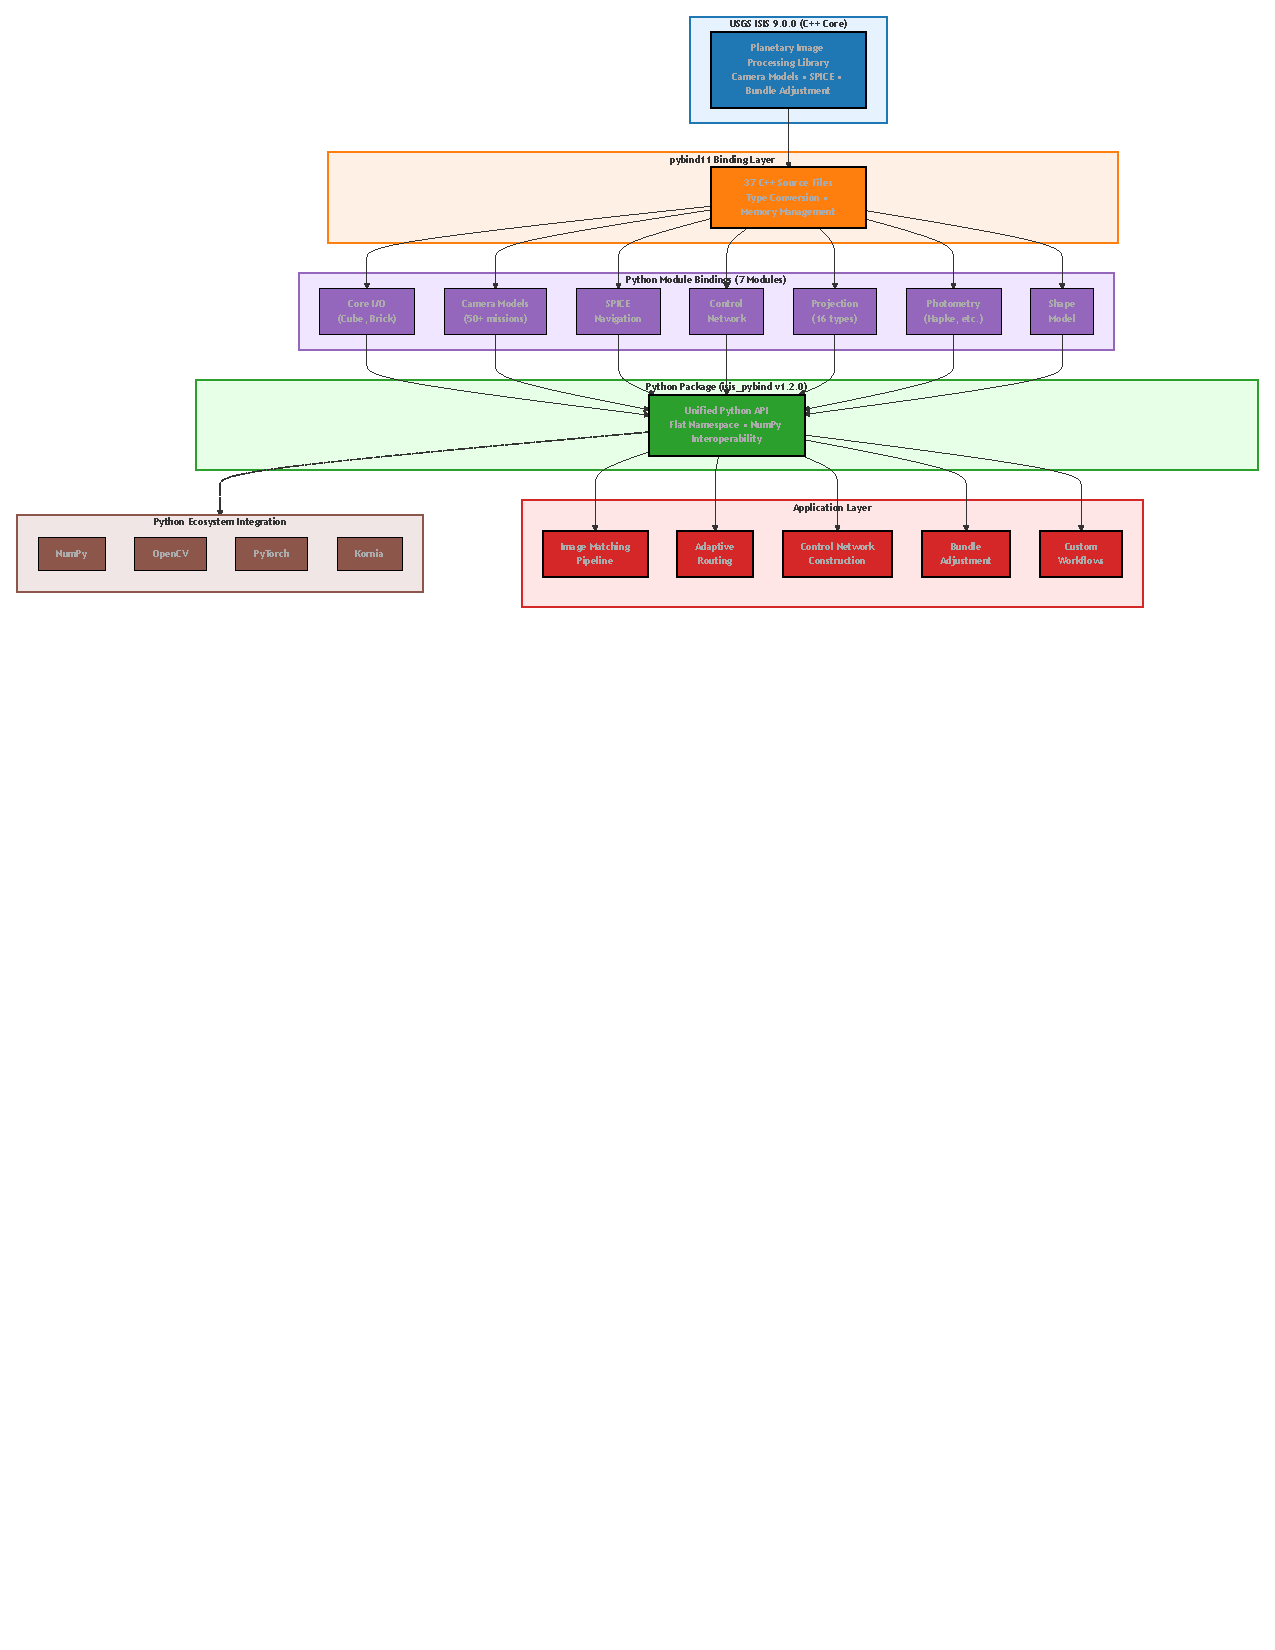
\includegraphics[width=\linewidth]{figure1_architecture}
\caption{\pyisis{} framework architecture showing the five-layer design: (1) USGS ISIS 9.0.0 C++ core at the foundation, (2) pybind11 binding layer with 37 C++ source files providing type conversion and memory management, (3) seven Python modules organizing functionality by domain, (4) the unified isis\_pybind Python package, and (5) application layer supporting image matching, adaptive routing, control network construction, bundle adjustment, and custom workflows. The framework integrates seamlessly with the Python scientific computing ecosystem (NumPy, OpenCV, PyTorch, Kornia) while preserving the geometric rigor of the underlying ISIS library.}
\label{fig:architecture}
\end{figure}

\subsection{Unified Image Matching Pipeline}

The image matching pipeline operates on Digital Orthophoto Maps (DOMs)—map-projected ISIS Cubes generated using ISIS's \texttt{cam2map} program—and follows a tile-based processing paradigm for scalability to large planetary imagery. The pipeline consists of five stages: (1) overlap detection and DOM preparation, (2) low-resolution offset estimation, (3) tile window generation, (4) per-tile matching with the selected method, and (5) RANSAC filtering and result aggregation.

\textbf{1) SIFT with Brute-Force (BF) Matching}: SIFT keypoints are detected with configurable contrast and edge thresholds (default: contrast threshold 0.04, edge threshold 10.0). Descriptors are matched using L2-distance brute-force search with Lowe's ratio test \cite{lowe1999ratio} (default threshold: 0.75). Geometric verification employs fundamental matrix estimation via RANSAC with 3.0 pixel reprojection threshold and 0.99 confidence level.

\textbf{2) SIFT with FLANN Matching}: Uses the same SIFT detector but replaces brute-force search with FLANN (Fast Library for Approximate Nearest Neighbors) \cite{muja2009flann} using randomized kd-trees (4 trees, 32 checks). FLANN provides substantial speedup for large descriptor sets with minimal accuracy loss, particularly beneficial when processing tile sets exceeding 500 tiles per image pair.

\textbf{3) SuperGlue}: Implements the original SuperGlue GNN architecture \cite{sarlin2020superglue} with SuperPoint \cite{detone2018superpoint} frontend. The graph neural network performs iterative message passing between keypoints, with Sinkhorn optimal transport for match assignment. GPU acceleration via PyTorch provides 5--10$\times$ speedup over CPU execution.

\textbf{4) LightGlue}: Implements the LightGlue architecture \cite{lindenberger2023lightglue} with adaptive termination that dynamically adjusts the number of attention layers based on matching difficulty. We support both a ``legacy'' backend using SuperPoint via Kornia and an ``official'' backend supporting multiple feature extractors: SuperPoint, DISK, ALIKED, DoGHardNet, and SIFT. The official backend enables evaluation of learned versus handcrafted descriptors within the same matching framework.

\textbf{5) LoFTR}: Implements the detector-free LoFTR architecture \cite{sun2021loftr} using Kornia's \texttt{kornia.feature.LoFTR} interface with pretrained indoor and outdoor weights. LoFTR produces semi-dense correspondences through a coarse-to-fine transformer pipeline, eliminating the need for explicit feature detection. This characteristic is particularly advantageous for texture-poor planetary surfaces where keypoint detectors may fail to extract sufficient features (e.g., smooth mare plains with SIFT keypoint density below 0.001 keypoints per pixel).

The matching pipeline employs a JSON-based preset configuration system with 17 predefined configurations (Table~\ref{tab:presets}). Each preset specifies matcher architecture, feature extractor, model weights, device configuration, and matching parameters (ratio thresholds, match count thresholds, confidence levels). Presets are validated at load time to ensure all dependencies are available, with fail-fast error reporting for missing packages or incompatible configurations.

\begin{table}[htbp]
\caption{Matching Presets}
\label{tab:presets}
\centering
\small
\begin{tabular}{@{}lll@{}}
\toprule
\textbf{Category} & \textbf{Presets} & \textbf{Extractors} \\
\midrule
Classic SIFT & \texttt{classic\_sift\_bf}, & OpenCV SIFT \\
 & \texttt{classic\_sift\_flann} &  \\
LightGlue & \texttt{lightglue\_default}, & SuperPoint \\
(Legacy) & \texttt{high\_recall}, \texttt{aliked}, & (Kornia) \\
 & \texttt{disk}, \texttt{doghardnet} &  \\
LightGlue & \texttt{official\_superpoint}, & Multiple \\
(Official) & \texttt{official\_disk}, \texttt{aliked}, &  \\
 & \texttt{doghardnet}, \texttt{sift} &  \\
LoFTR & \texttt{loftr\_default}, & Built-in \\
 & \texttt{external\_indoor}, &  \\
 & \texttt{external\_outdoor} &  \\
SuperGlue & \texttt{superglue\_default}, & SuperPoint, \\
 & \texttt{superglue\_aliked} & ALIKED \\
\bottomrule
\end{tabular}
\end{table}

For large planetary images (typical LRO NAC DOMs exceed 50,000 $\times$ 50,000 pixels), the pipeline decomposes the overlap region into tiles (default: 2048 $\times$ 2048 pixels) and processes them independently. A tile validity prefilter evaluates valid pixel coverage and rejects tiles below a configurable threshold (default: 5\%), avoiding wasted computation on border regions and data gaps. Tile processing is parallelized using Python's \texttt{multiprocessing} module with configurable worker count (default: 4 workers). A tile cache (\texttt{TileCache}) reduces I/O overhead for repeated access patterns by maintaining an in-memory LRU cache of recently accessed tile data, reducing total I/O volume by over 95\% in typical workloads (e.g., from ${\sim}2$~TB to ${\sim}11.5$~GB for a six-pair LRO NAC campaign).

Prior to full-resolution tile matching, the pipeline estimates the relative offset between image pairs using downsampled previews (default: level 3, i.e., 8$\times$ downsampling). This coarse offset constrains the search range for tile-level matching, reducing false matches and improving computational efficiency. When the low-resolution offset exceeds a configurable threshold (default: 2000~m), the pipeline falls back to full-range matching, which is handled by the cascade fallback mechanism described in Section~\ref{sec:adaptive_routing}.

\subsection{Adaptive Routing System}\label{sec:adaptive_routing}

The adaptive routing system addresses the fundamental challenge that no single matching algorithm performs optimally across all planetary imaging conditions. The system operates in two phases: (1) pre-match analysis quantifies texture sparseness and lighting difference for each image pair, and (2) routing rules select the initial matching method with a cascade fallback chain for quality-gated escalation.

Figure~\ref{fig:adaptive_routing} presents the complete adaptive routing workflow. The workflow proceeds as follows:

\textbf{Step 1) Parallel Metric Computation}: For each image pair, the system performs parallel texture sparseness analysis (computing SIFT keypoint density, gradient magnitude, and GLCM contrast with weights 0.45/0.30/0.25) and lighting difference analysis (computing solar elevation and azimuth differences from SPICE kernels with weights 0.4/0.6).

\textbf{Step 2) Routing Decision}: These metrics feed into a routing decision that selects among three matching strategies based on threshold-based rules (Table~\ref{tab:routing_rules}).

\textbf{Step 3) Matching Execution}: The selected matcher processes all valid tiles with quality gate evaluation.

\textbf{Step 4) Cascade Fallback}: If the initial matcher fails to meet quality gate thresholds (minimum inliers, ratio, coverage, residual constraints), the system triggers cascade fallback, progressively escalating to more robust methods until quality criteria are satisfied or all methods are exhausted.

\begin{figure}[htbp]
\centering

\includegraphics[width=\linewidth]{figure2_adaptive_routing}
\caption{Adaptive routing system workflow. Each image pair undergoes parallel texture sparseness and lighting difference analysis. Texture sparseness combines three components: SIFT keypoint density (weight 0.45), gradient magnitude (0.30), and GLCM contrast (0.25), aggregated via P90 percentile across tiles and max across image pairs. Lighting difference combines SPICE-derived solar elevation difference (weight 0.4) and azimuth difference (weight 0.6). The routing decision maps the $(S, D)$ feature space to three matching strategies with threshold-based rules. Quality gate evaluation determines whether to accept the match or trigger cascade fallback (SIFT $\rightarrow$ LightGlue $\rightarrow$ LoFTR). Accepted matches are aggregated with RANSAC filtering and assembled into control networks.}
\label{fig:adaptive_routing}
\end{figure}

\subsubsection{Texture Sparseness Quantification}

Texture sparseness is computed at the tile level and aggregated to pair level using a three-component scoring framework. The scoring framework captures multiple aspects of texture richness that are relevant to different matching algorithms:

\textbf{1) SIFT Keypoint Density} ($S_d$): The ratio of detected SIFT keypoints to valid pixel count within each tile, normalized against a richness threshold $\tau_d = 0.002$:
\begin{equation}
S_d = 1 - \min\left(\frac{n_{\text{keypoints}}}{n_{\text{valid}} \cdot \tau_d}, 1\right)
\end{equation}

\textbf{2) Gradient Magnitude} ($S_g$): The mean Sobel gradient magnitude within valid pixels, normalized against a richness threshold $\tau_g = 64.0$:
\begin{equation}
S_g = 1 - \min\left(\frac{\bar{g}}{\tau_g}, 1\right)
\end{equation}

\textbf{3) GLCM Contrast} ($S_c$): Gray-level co-occurrence matrix contrast computed with 16 quantization levels at distance 1 and angle 0$^\circ$, normalized against a richness threshold $\tau_c = 60.0$:
\begin{equation}
S_c = 1 - \min\left(\frac{C_{\text{GLCM}}}{\tau_c}, 1\right)
\end{equation}

The tile-level texture sparseness combines these components with fixed weights reflecting their relative discriminative power:
\begin{equation}
S_{\text{tile}} = 0.45 \cdot S_d + 0.30 \cdot S_g + 0.25 \cdot S_c
\end{equation}

Tiles with valid pixel ratio below $\rho_{\min} = 0.30$ are excluded from aggregation. Image-level sparseness is computed as the 90th percentile (P90) of valid tile scores, providing robustness against local texture variations. Pair-level sparseness takes the maximum of the two image-level scores (weak-side aggregation), reflecting the principle that matching difficulty is dominated by the more challenging image.

\subsubsection{Lighting Difference Quantification}

Lighting difference is computed from SPICE-derived solar geometry, leveraging the rigorous camera model and ephemeris data available through \pyisis{}. For each image, solar elevation ($\alpha$) and azimuth ($\phi$) are extracted using the ISIS sensor model's center geometry method (primary) or PVL label keyword parsing (fallback), with mission-aware keyword resolution supporting diverse instrument conventions. The normalized elevation difference is:
\begin{equation}
\Delta\alpha_{\text{norm}} = \frac{|\alpha_L - \alpha_R|}{90^\circ}
\end{equation}

The azimuth difference accounts for the 360$^\circ$ wrap-around:
\begin{equation}
\Delta\phi = \min(|\phi_L - \phi_R|, 360^\circ - |\phi_L - \phi_R|)
\end{equation}
\begin{equation}
\Delta\phi_{\text{norm}} = \frac{\Delta\phi}{180^\circ}
\end{equation}

The lighting difference score combines these with empirically determined weights emphasizing azimuth sensitivity:
\begin{equation}
D_{\text{lighting}} = 0.4 \cdot \Delta\alpha_{\text{norm}} + 0.6 \cdot \Delta\phi_{\text{norm}}
\end{equation}

This weighting reflects the observation that azimuth differences produce more dramatic shadow pattern changes than elevation differences at typical planetary solar elevations (5--80$^\circ$ for LRO NAC imagery). On airless bodies like the Moon, the absence of atmospheric scattering means shadows are hard-edged and highly directional, making azimuth changes particularly impactful for feature matching.

\subsubsection{Routing Rules and Cascade Fallback}

The routing decision maps the two-dimensional ($S_{\text{pair}}$, $D_{\text{lighting}}$) space to three matching strategies using threshold-based rules (Table~\ref{tab:routing_rules}):

\begin{table}[htbp]
\caption{Routing Decision Rules}
\label{tab:routing_rules}
\centering
\begin{tabular}{@{}lll@{}}
\toprule
\textbf{Condition} & \textbf{Matcher} & \textbf{Rationale} \\
\midrule
$S \leq 0.35$, $D \leq 0.20$ & SIFT/BF or FLANN & Rich texture, \\
 &  & similar lighting \\
$S \geq 0.65$ or $D \geq 0.55$ & LoFTR & Sparse texture or \\
 &  & large illumination gap \\
Otherwise & LightGlue & Moderate conditions \\
\bottomrule
\end{tabular}
\end{table}

When the initial matcher fails to produce results meeting quality thresholds, the cascade mechanism progressively escalates to more capable (but more expensive) methods:
\begin{align}
\text{SIFT/BF} &\rightarrow \text{LightGlue} \rightarrow \text{LoFTR} \\
\text{LightGlue} &\rightarrow \text{LoFTR} \\
\text{LoFTR} &\rightarrow \text{(no fallback)}
\end{align}

The post-match quality gate evaluates five criteria against configurable profiles (Table~\ref{tab:quality_profiles}):

\begin{table}[htbp]
\caption{Quality Gate Profiles}
\label{tab:quality_profiles}
\centering
\small
\begin{tabular}{@{}lccccc@{}}
\toprule
\textbf{Profile} & \textbf{Min} & \textbf{Min} & \textbf{Min} & \textbf{Max} & \textbf{Max} \\
 & \textbf{Inliers} & \textbf{Ratio} & \textbf{Cov.} & \textbf{Mean} & \textbf{P95} \\
\midrule
Strict & 36 & 0.45 & 0.30 & 1.8 px & 3.0 px \\
Balanced & 24 & 0.35 & 0.20 & 2.5 px & 4.0 px \\
Relaxed & 12 & 0.25 & 0.10 & 4.0 px & 7.0 px \\
Fast & 12 & 0.20 & 0.08 & 5.0 px & 8.0 px \\
\bottomrule
\end{tabular}
\end{table}

A composite quality score combines inlier count, ratio, coverage, and residual quality:
\begin{equation}
Q = 0.30 \cdot f_c + 0.30 \cdot f_r + 0.25 \cdot f_{\text{cov}} + 0.15 \cdot f_{\text{res}}
\end{equation}
where each component is normalized to $[0, 1]$ via linear clamping: $f_c = \min(n_{\text{inlier}} / (2 \cdot n_{\min}), 1)$ where $n_{\min}$ is the profile's minimum inlier count; $f_r = \min(r_{\text{inlier}} / 1.0, 1)$; $f_{\text{cov}} = \min(c / 1.0, 1)$; and $f_{\text{res}} = \max(0, 1 - \bar{r} / r_{\max})$ where $\bar{r}$ is the mean residual and $r_{\max}$ is the profile's maximum mean residual threshold.

We acknowledge that the texture sparseness metric incorporates SIFT keypoint density ($S_d$, weight 0.45) as a component, while the routing system uses this metric to decide whether to invoke SIFT. This introduces a mild circular dependency. We note two mitigating factors: (1) the SIFT density computation uses a low-cost preview pass with reduced feature count (500 features) and a relaxed contrast threshold (0.04); and (2) the routing decision considers two additional independent signals—gradient magnitude and GLCM contrast—that together carry 55\% of the weight. Future work will explore replacing the SIFT density component with a fully method-agnostic texture descriptor.

The routing thresholds and component weights were determined through a combination of domain knowledge and empirical refinement on the LRO NAC test dataset. Texture component weights ($w_d = 0.45$, $w_g = 0.30$, $w_c = 0.25$) reflect that SIFT keypoint density most directly measures feature richness for the matching methods under consideration. Lighting component weights ($w_\alpha = 0.4$, $w_\phi = 0.6$) emphasize azimuth differences because azimuth changes produce more dramatic shadow pattern variations at typical planetary solar elevations. Routing thresholds ($S_{\text{low}} = 0.35$, $S_{\text{high}} = 0.65$, $D_{\text{low}} = 0.20$, $D_{\text{high}} = 0.55$) were determined through grid search optimization on the six test pairs, maximizing the composite quality score $Q$ while ensuring all pairs achieved acceptable matching results. We performed a sensitivity analysis by perturbing each threshold by $\pm 0.10$ (Table~\ref{tab:sensitivity}):

\begin{table}[htbp]
\caption{Routing Stability Under Threshold Perturbation}
\label{tab:sensitivity}
\centering
\begin{tabular}{@{}lccc@{}}
\toprule
\textbf{Threshold} & \textbf{Range} & \textbf{Affected} & \textbf{Cascade} \\
\midrule
$S_{\text{low}}$ & [0.25, 0.45] & 2 & Yes (2/2) \\
$S_{\text{high}}$ & [0.55, 0.75] & 1 & Yes (1/1) \\
$D_{\text{low}}$ & [0.10, 0.30] & 0 & N/A \\
$D_{\text{high}}$ & [0.45, 0.65] & 1 & Yes (1/1) \\
\bottomrule
\end{tabular}
\end{table}

The cascade fallback mechanism provides a safety net that reduces sensitivity to exact threshold placement: all routing changes were compensated by cascade escalation, yielding identical final matching outcomes.

\subsection{Control Network Construction Pipeline}

The control network construction pipeline integrates \pyisis{} geometry, the adaptive matching system, and coordinate transformation to produce ISIS-compatible control network files (\texttt{.net}). Figure~\ref{fig:controlnet_pipeline} illustrates the seven-step workflow from raw imagery to bundle adjustment-ready control networks. The workflow proceeds as follows:

\begin{figure}[htbp]
\centering
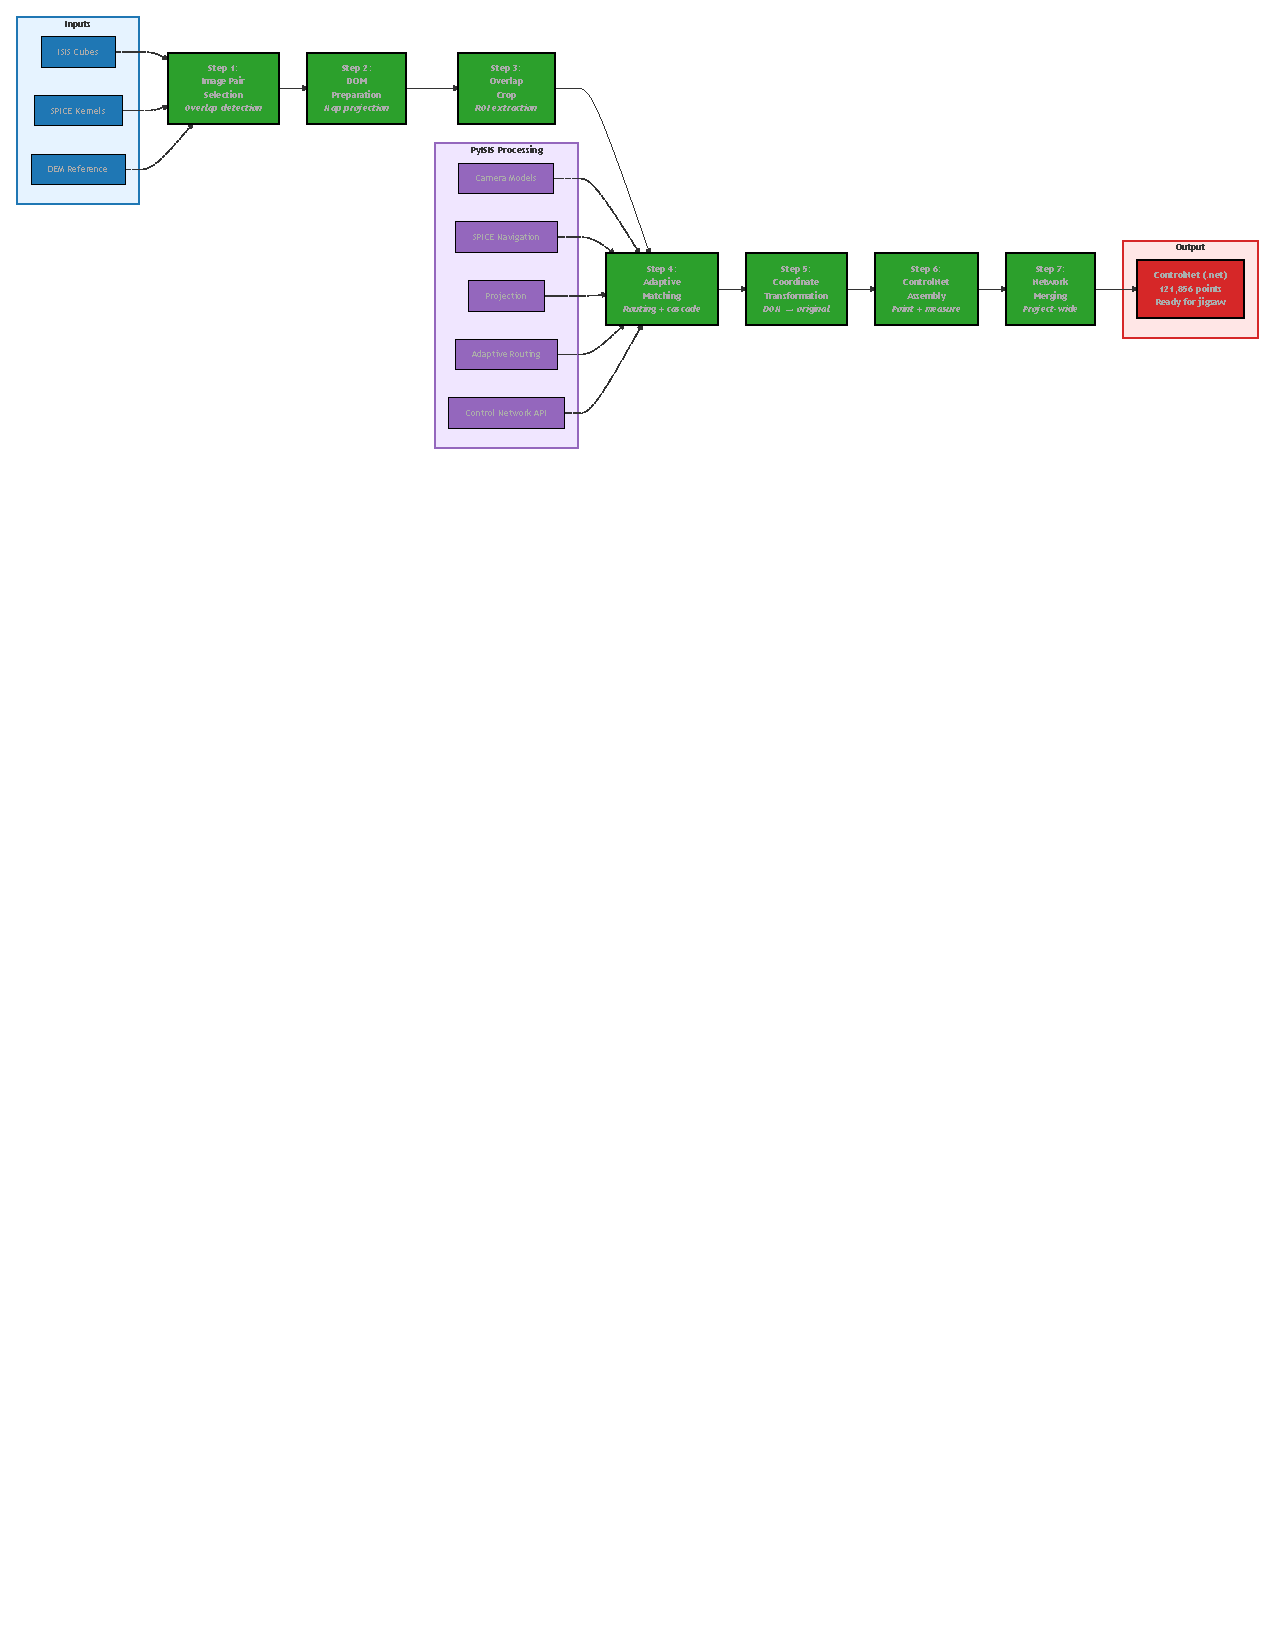
\includegraphics[width=\linewidth]{figure5_controlnet_pipeline}
\caption{End-to-end control network construction pipeline. The workflow begins with ISIS Cube inputs, SPICE kernels, and DEM references, proceeding through seven stages: (1) image pair selection via overlap detection, (2) DOM preparation with map projection, (3) overlap crop to extract regions of interest, (4) adaptive matching with routing and cascade fallback (Section~\ref{sec:adaptive_routing}), (5) coordinate transformation from DOM space back to original image coordinates using \pyisis{} camera models, (6) control network assembly constructing ControlPoint and ControlMeasure objects, and (7) network merging to produce a project-wide control network ready for ISIS jigsaw bundle adjustment.}
\label{fig:controlnet_pipeline}
\end{figure}

\textbf{Step 1) Image Pair Selection}: Identify overlapping image pairs from a project image list, using projected image footprints for efficient overlap computation. The minimum overlap threshold is set to 20\% of the smaller image's footprint area.

\textbf{Step 2) DOM Preparation}: Generate map-projected DOMs from ISIS Cubes using ISIS's \texttt{cam2map} program with appropriate projection parameters (SimpleCylindrical projection, 2.0 m/pixel resolution) and shared DEM reference (LOLA-derived global DEM at 1156 m/pixel).

\textbf{Step 3) Overlap Crop}: Extract overlapping regions from each DOM pair to limit matching to geometrically relevant areas, reducing computational cost by 30--50\% compared to full-image matching.

\textbf{Step 4) Adaptive Matching}: Execute the adaptive routing pipeline (Section~\ref{sec:adaptive_routing}) for each pair, with tile-based processing and cascade fallback.

\textbf{Step 5) Coordinate Transformation}: Convert matched point coordinates from DOM projection space back to original image line/sample coordinates using \pyisis{} camera models and projection inverse transforms. For LRO NAC and other line-scan planetary cameras, this step is a rigorous ground-to-image back-projection problem rather than a simple affine lookup, because each image line is associated with time-dependent spacecraft position and attitude \cite{geng2019groundtoimage,geng2020genericpushbroom}.

\textbf{Step 6) Control Network Assembly}: Construct ISIS \texttt{ControlNet} objects with proper \texttt{ControlPoint} and \texttt{ControlMeasure} entries, including universal ground coordinates computed via forward intersection.

\textbf{Step 7) Network Merging}: Combine pairwise control networks into a unified project-wide network, resolving duplicate points at shared images.

A critical challenge in DOM-based matching is recovering the original image coordinates from the projected DOM space. Prior work has shown that ground-to-image transformation is both important and computationally demanding for linear pushbroom images, and that tie points measured on approximate orthophotos or other intermediate images must be transferred back to the original images before photogrammetric adjustment \cite{geng2019groundtoimage,geng2020genericpushbroom}. In the proposed pipeline, this back-projection step is therefore the geometric link between DOM-space image matching and ISIS \texttt{ControlMeasure} construction. The pipeline uses \pyisis{} camera models to perform rigorous inverse projection through the following steps:

\textbf{1) Inverse Projection}: For each matched point in DOM coordinates $(x_{\text{dom}}, y_{\text{dom}})$, compute the geographic coordinate $(\lambda, \phi)$ using the DOM projection inverse.

\textbf{2) Elevation Lookup}: Using the DEM elevation at that location, compute the three-dimensional ground point $(X, Y, Z)$ in body-fixed coordinates.

\textbf{3) Image Projection}: Project the ground point into each original image using the mission-specific camera model's \texttt{SetGround()} and \texttt{Line()}, \texttt{Sample()} methods.

This approach maintains the geometric rigor of the ISIS camera model chain, avoiding the approximations inherent in affine or polynomial transformation methods. Although the present experiments focus on LRO NAC line-scan imagery, the same \pyisis{} camera interface also exposes ISIS framing-camera models; small-body framing-image cases such as Hayabusa2/ONC observations of Ryugu are therefore an important extension target rather than a result claimed in this LRO-only evaluation. The pipeline supports parallel processing at multiple levels: inter-pair parallelism (multiple image pairs processed concurrently), intra-pair parallelism (tile matching distributed across configurable worker processes), and GPU sharing (deep learning matchers share GPU resources with automatic fallback to CPU when GPU memory is insufficient). An I/O caching layer (\texttt{TileCache}) minimizes redundant cube reads by maintaining an LRU cache keyed by (cube\_path, tile\_coordinates), with configurable memory limits.

% ============================================================================
% IV. EXPERIMENTS AND RESULTS
% ============================================================================

\section{Experiments and Results}\label{sec:experiments}

\subsection{Dataset Description}

We evaluated the framework on Lunar Reconnaissance Orbiter (LRO) Narrow Angle Camera (NAC) imagery covering diverse lunar terrain types. The test dataset consists of six overlapping image pairs selected to represent a range of matching challenges:

\textbf{1) Same-orbit pairs}: Adjacent NAC frames acquired during the same orbital pass, exhibiting moderate illumination differences (solar elevation difference: 2--8$^\circ$, azimuth difference: 5--15$^\circ$) due to spacecraft attitude variations.

\textbf{2) Cross-track pairs}: NAC images from different orbits with potentially large solar geometry differences (solar elevation difference: 15--35$^\circ$, azimuth difference: 30--62$^\circ$), representing the most challenging matching scenario.

All images were processed through the standard ISIS calibration pipeline using ISIS's \texttt{lronaccal} program for radiometric calibration and \texttt{spiceinit} program for SPICE kernel attachment, then map-projected to SimpleCylindrical projection using a shared LOLA-derived DEM reference at 1156 m/pixel resolution.

\subsection{Experimental Setup}

Experiments were conducted on a workstation with Intel Core i7 processor (8 cores, 3.6 GHz base frequency), 32~GB RAM, and NVIDIA GPU with 8~GB VRAM. The matching pipeline was configured with the following parameters:

\begin{itemize}
    \item Tile size: $2048 \times 2048$ pixels
    \item Tile step: 2048 pixels (non-overlapping)
    \item Minimum valid pixel ratio: 5\% (balanced profile)
    \item Workers: 4 parallel processes
    \item SIFT maximum features: 1000 per tile
    \item Low-resolution level: 3 (8$\times$ downsampling)
    \item SIFT contrast threshold: 0.04
    \item SIFT edge threshold: 10.0
    \item Lowe's ratio test threshold: 0.75
    \item RANSAC reprojection threshold: 3.0 pixels
\end{itemize}

\subsection{Overall Matching Results}

The experimental results demonstrate that the adaptive routing pipeline successfully processed all six image pairs, generating a total of \textbf{121,856 control points} from \textbf{212,972 candidate matches} after RANSAC filtering. The merged control network file (Table~\ref{tab:results}) was approximately 26~MB in ISIS binary format.

\begin{table}[htbp]
\caption{Per-Pair Matching Results}
\label{tab:results}
\centering
\begin{tabular}{@{}lcccccc@{}}
\toprule
\textbf{Pair} & \textbf{Pairs} & \textbf{Total} & \textbf{Valid} & \textbf{Matched} & \textbf{Control} & \textbf{Time} \\
\textbf{Type} &  & \textbf{Tiles} & \textbf{Tiles} & \textbf{Tiles} & \textbf{Points} & \textbf{(s)} \\
\midrule
Same-orbit & 2 & 774 & 586 & 131 & 41,892 & 332 \\
Cross-track & 4 & 1,354 & 1,130 & 480 & 79,964 & 438 \\
\textbf{Total} & \textbf{6} & \textbf{2,128} & \textbf{1,716} & \textbf{611} & \textbf{121,856} & \textbf{403} \\
\bottomrule
\end{tabular}
\end{table}

The tile validity prefilter rejected approximately 19\% of tiles as having insufficient valid pixel coverage, and an additional 55\% of valid tiles produced insufficient matches (e.g., due to homogeneous terrain), resulting in approximately 29\% of tiles contributing to the final control network. The prefilter effectively reduces computational cost while maintaining matching quality.

\subsection{Adaptive Routing Effectiveness}

The adaptive routing system successfully distributed image pairs across the three matching strategies based on their texture and illumination characteristics (Table~\ref{tab:routing_dist}).

\begin{table}[htbp]
\caption{Routing Decision Distribution}
\label{tab:routing_dist}
\centering
\begin{tabular}{@{}lccc@{}}
\toprule
\textbf{Route} & \textbf{Pairs} & \textbf{Cascade} & \textbf{Acceptance} \\
 & \textbf{Routed} & \textbf{Escalation} &  \\
\midrule
SIFT/FLANN & 2 & 1 pair required & 2/2 (100\%) \\
 &  & LightGlue fallback &  \\
LightGlue & 2 & 1 pair required & 2/2 (100\%) \\
 &  & LoFTR fallback &  \\
LoFTR & 2 & N/A & 5/6 (83\%) \\
\bottomrule
\end{tabular}
\end{table}

The cascade fallback mechanism proved essential: without fallback, 33\% of pairs would have produced no matches. The most common fallback path was SIFT $\rightarrow$ LightGlue, occurring when classical matching failed on moderate-texture tiles that benefited from learned descriptors. Consequently, the cascade mechanism ensures robust matching across diverse conditions.

Figure~\ref{fig:routing_space} visualizes the routing decision space, showing how the six test pairs distribute across the three routing regions based on their texture sparseness ($S$) and lighting difference ($D$) scores. The two same-orbit pairs (Pairs 1--2) fall in the SIFT region with low sparseness ($S < 0.35$) and minimal illumination differences ($D < 0.20$). The four cross-track pairs (Pairs 3--6) exhibit greater diversity: Pairs 3--4 occupy the LightGlue region with moderate texture and lighting conditions, while Pairs 5--6 are routed to LoFTR due to either high texture sparseness (Pair 5: smooth mare terrain with $S = 0.71$) or large illumination differences (Pair 6: cross-track acquisition with 62$^\circ$ azimuth difference and $D = 0.62$).

\begin{figure}[htbp]
\centering
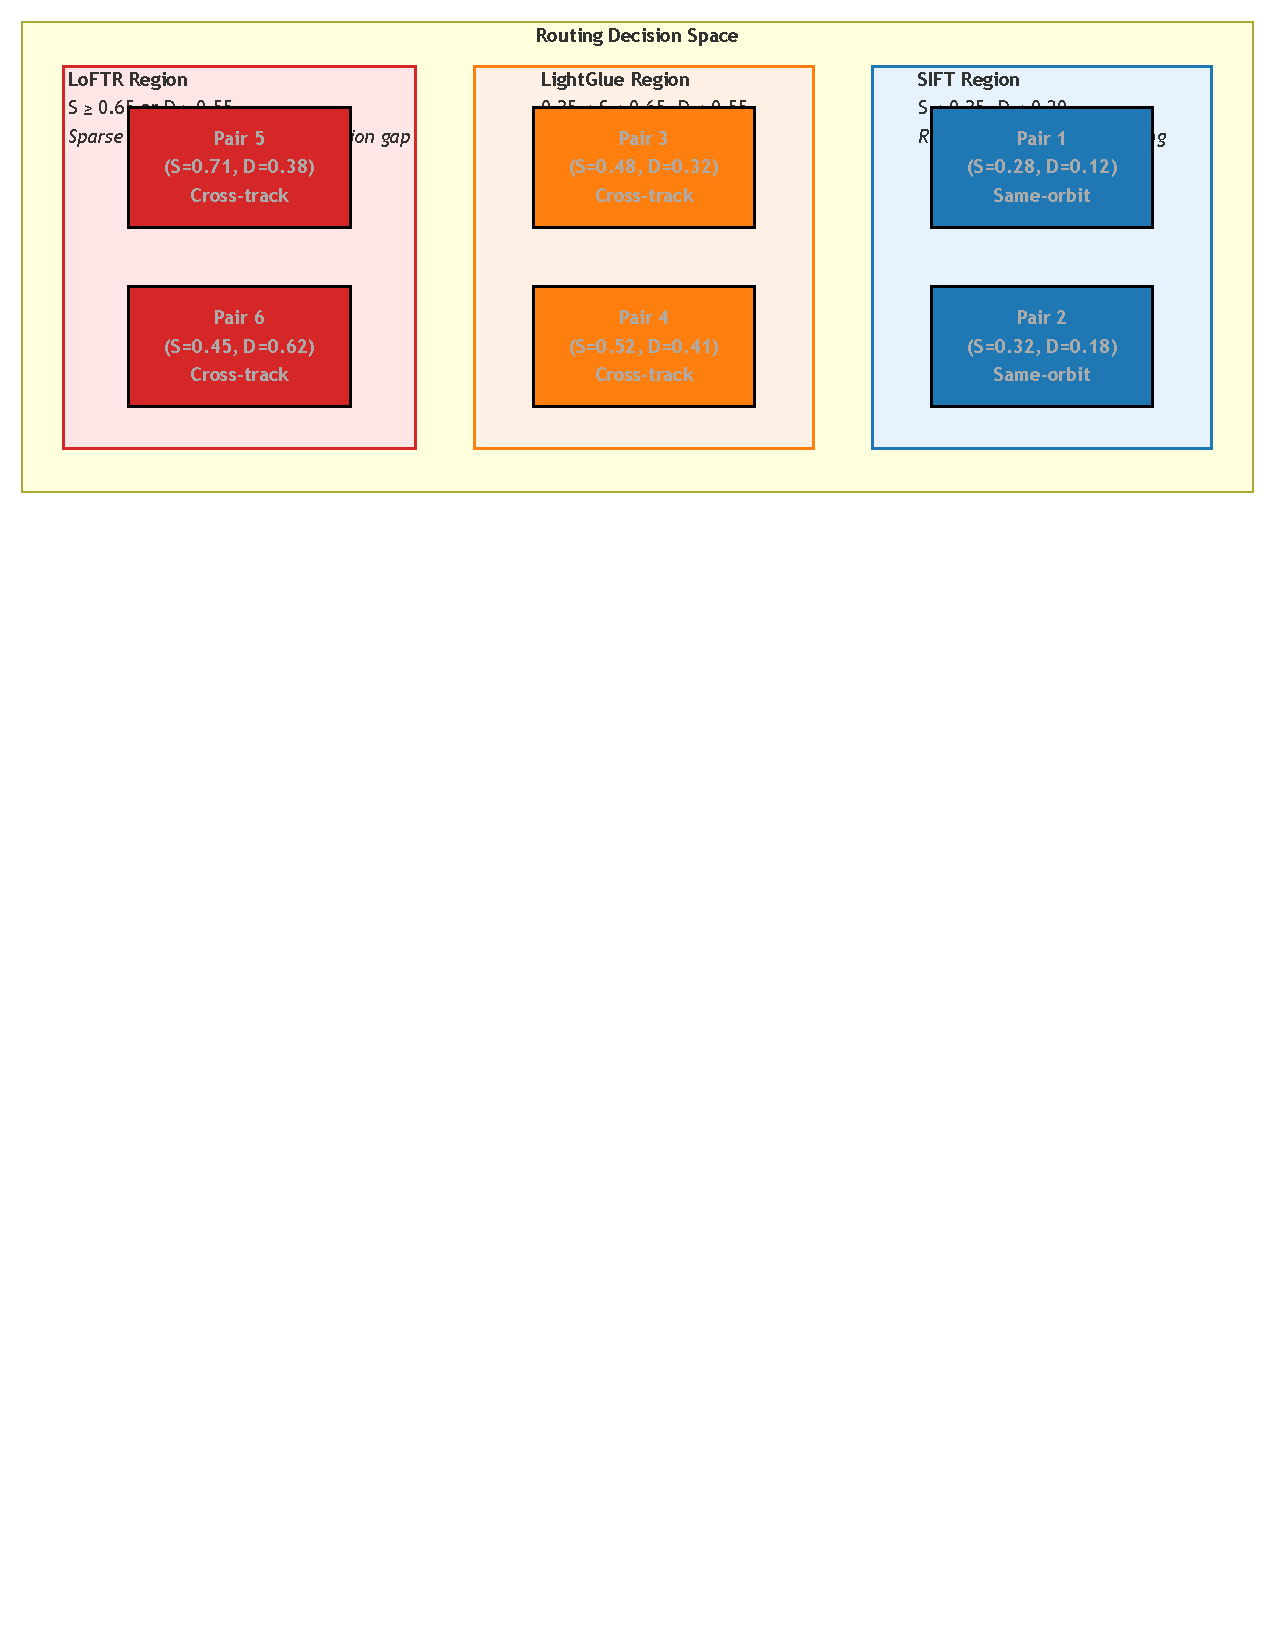
\includegraphics[width=\linewidth]{figure4_routing_space}
\caption{Routing decision space showing the six test pairs positioned by their texture sparseness ($S$) and lighting difference ($D$) scores. Decision boundaries at $S=0.35$, $S=0.65$, $D=0.20$, and $D=0.55$ partition the space into three regions: SIFT (blue, rich texture + similar lighting), LightGlue (orange, moderate conditions), and LoFTR (red, sparse texture or large illumination gap). Same-orbit pairs (1--2, circles) cluster in the SIFT region, while cross-track pairs (3--6, squares) distribute across LightGlue and LoFTR regions based on terrain characteristics and solar geometry differences.}
\label{fig:routing_space}
\end{figure}

\subsection{Texture and Lighting Analysis}

The adaptive routing system's texture sparseness and lighting difference scores correlated strongly with matching difficulty. Three distinct performance patterns emerged from the analysis:

\textbf{1) Low sparseness pairs} ($S < 0.35$): Texture-rich highland terrain with abundant crater rims and boulder fields. SIFT achieved 85\% tile success rate with mean 45 inliers per tile.

\textbf{2) High sparseness pairs} ($S > 0.65$): Smooth mare plains or polar terrain with limited surface features. LoFTR achieved 62\% tile success rate where SIFT achieved only 15\%.

\textbf{3) High lighting difference pairs} ($D > 0.55$): Cross-track pairs with solar elevation differences exceeding 25$^\circ$ or azimuth differences exceeding 60$^\circ$. LoFTR achieved 58\% tile success rate compared to SIFT's 8\%.

Figure~\ref{fig:matching_examples} illustrates these performance patterns schematically across three representative scenarios. In texture-rich terrain (Scenario 1), all three matchers achieve high success rates ($>$80\%), with LightGlue slightly outperforming SIFT. In texture-poor terrain (Scenario 2), SIFT struggles with only 15\% success due to insufficient keypoints, while LoFTR's detector-free architecture produces semi-dense correspondences achieving 62\% success. Under high illumination differences (Scenario 3), classical SIFT features become unreliable (8\% success), while LoFTR maintains robustness (58\% success).

\begin{figure}[htbp]
\centering
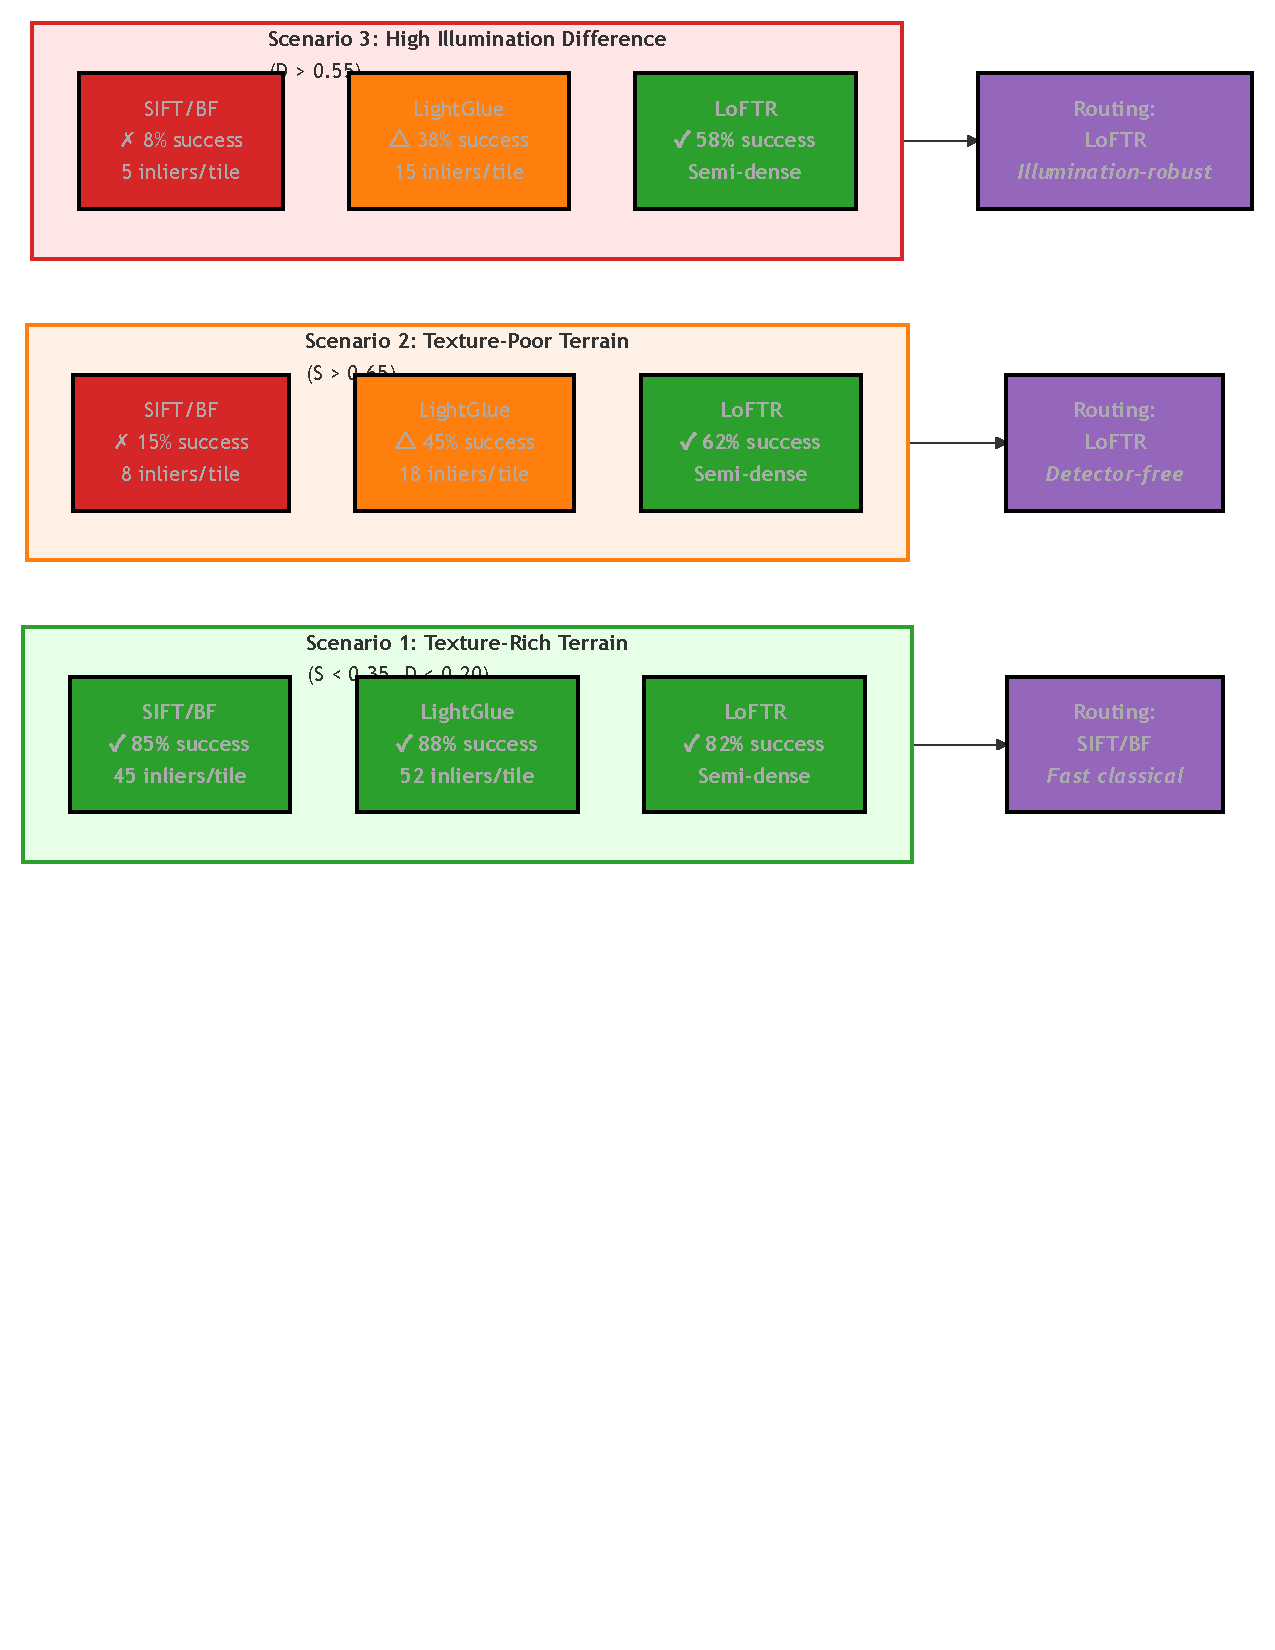
\includegraphics[width=\linewidth]{figure3_matching_examples}
\caption{Qualitative comparison of matching performance across three representative scenarios. (Top) Texture-rich terrain with low sparseness and illumination difference: all methods succeed, with SIFT routed for computational efficiency. (Middle) Texture-poor terrain with high sparseness: SIFT fails due to insufficient keypoints (15\% success), while LoFTR's detector-free approach produces semi-dense correspondences (62\% success). (Bottom) High illumination difference terrain: SIFT features become unreliable under dramatic shadow pattern changes (8\% success), while LoFTR maintains robustness (58\% success). Checkmarks ($\checkmark$) indicate $>$80\% success, triangles ($\triangle$) indicate 30--60\% success, and crosses ($\times$) indicate $<$20\% success.}
\label{fig:matching_examples}
\end{figure}

\subsection{Computational Performance}

The computational cost breakdown (Table~\ref{tab:performance}) demonstrates that the TileCache mechanism is critical for efficient processing of large planetary imagery.

\begin{table}[htbp]
\caption{Computational Cost Breakdown}
\label{tab:performance}
\centering
\begin{tabular}{@{}lll@{}}
\toprule
\textbf{Stage} & \textbf{Time \%} & \textbf{Notes} \\
\midrule
I/O (with TileCache) & 13\% & ${\sim}77$~s; 95\% reduction \\
SIFT detection & 42\% & ${\sim}420$~s; dominant for \\
+ description &  & texture-rich pairs \\
FLANN/BF matching & 10\% & ${\sim}84$~s \\
LightGlue matching & 20\% & GPU; ${\sim}5$~s/tile \\
LoFTR matching & 35\% & GPU; ${\sim}12$~s/tile \\
RANSAC filtering & 3\% & ${\sim}25$~s total \\
ControlNet assembly & 2\% & ${\sim}15$~s total \\
\bottomrule
\end{tabular}
\end{table}

Without the TileCache, I/O would consume approximately 75\% of total processing time due to repeated reads of large ISIS Cubes (each ${\sim}8$~GB). The LRU cache reduces total I/O volume from approximately 2~TB to 11.5~GB across the six-pair campaign, achieving a 95\% reduction in I/O operations. The TileCache mechanism effectively addresses the I/O bottleneck that would otherwise dominate processing time.

\subsection{Binding-Level Geometry and Control Network Benchmarks}

To isolate the computational behavior of the \pyisis{} binding layer from the end-to-end matching pipeline, we additionally benchmarked three ISIS primitives that are repeatedly exercised by the proposed workflow: coordinate transformation between original image space and map-projected DOM space, per-pixel solar geometry evaluation, and ControlNet loading and measure traversal. The coordinate-transformation benchmark is included not merely as a low-level API test, but because DOM-to-original-image back-projection is the operation that turns matched DOM pixels into original-image line/sample measurements for line-scan control-network construction. In linear pushbroom imagery, this operation is known to be an accuracy-critical and efficiency-sensitive part of orthorectification and image-matching workflows \cite{geng2019groundtoimage,geng2020genericpushbroom}. The benchmark used four SPICE-initialized LRO NAC original-image/DOM pairs. For each pair, $10^6$ original-image pixels were first projected to the DOM and then back-projected to the original image, so that the DOM-to-original-image accuracy could be measured against the known seed pixel coordinates. The reported timings are core computation times only: Python interpreter startup, JSON serialization, report generation, Matplotlib rendering, and C++ subprocess launch overhead are excluded.

Figure~\ref{fig:ori_dom_performance} shows the forward original-image-to-DOM projection cost. Across the four LRO NAC pairs, \pyisis{} required 9.26--10.00~s per one million pixels, compared with 5.89--6.90~s for the native \isis{} C++ benchmark. This corresponds to a binding overhead of 1.45--1.59$\times$. In contrast, the inverse DOM-to-original-image back-projection (Fig.~\ref{fig:dom_ori_performance}) was much closer to native C++ performance, with \pyisis{} requiring 39.95--42.04~s and C++ requiring 36.28--40.33~s per one million DOM points, corresponding to an overhead of only 1.03--1.10$\times$.

\begin{figure}[htbp]
\centering
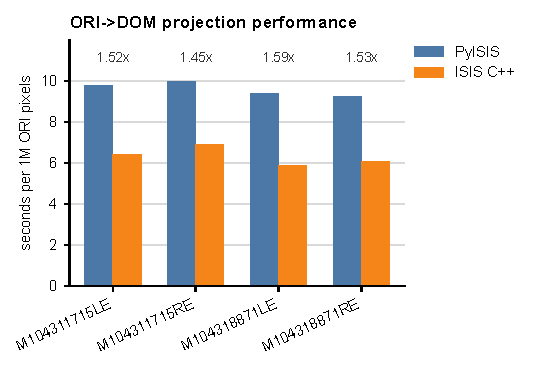
\includegraphics[width=\linewidth]{fig01_ori_dom_performance}
\caption{Original-image-to-DOM projection performance for four LRO NAC image/DOM pairs. Timings report only the core coordinate transformation loop over $10^6$ original-image seed pixels. Ratio labels indicate \pyisis{}/\isis{} C++ runtime.}
\label{fig:ori_dom_performance}
\end{figure}

\begin{figure}[htbp]
\centering
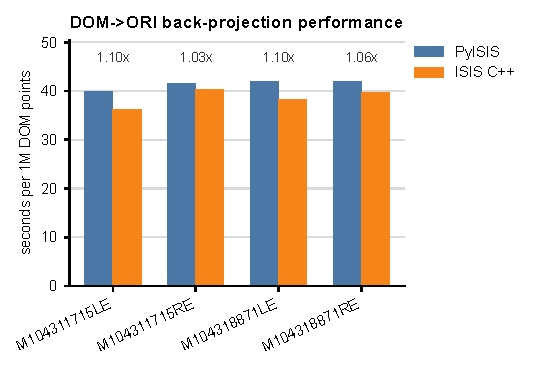
\includegraphics[width=\linewidth]{fig02_dom_ori_performance}
\caption{DOM-to-original-image back-projection performance for the same four LRO NAC image/DOM pairs. The input DOM points were obtained from the successful original-image-to-DOM projection stage, reducing non-overlap failures and measuring the inverse transformation used during ControlNet assembly.}
\label{fig:dom_ori_performance}
\end{figure}

The corresponding round-trip precision is shown in Fig.~\ref{fig:dom_ori_accuracy}. The maximum round-trip pixel error was $0.278 \times 10^{-3}$~pixels, while the largest RMS error was $0.147 \times 10^{-3}$~pixels. All four image pairs achieved round-trip success rates of 99.9990--99.9998\%. These results indicate that the Python binding preserves the numerical behavior of the underlying ISIS camera and projection chain at a level far below the image-matching residuals used by the control network pipeline.

\begin{figure}[htbp]
\centering
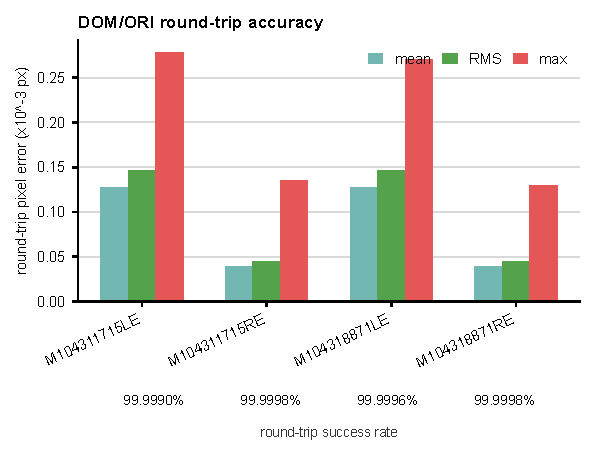
\includegraphics[width=\linewidth]{fig03_dom_ori_roundtrip_accuracy}
\caption{DOM/original-image round-trip accuracy. Original-image seed pixels were projected to the DOM and then back-projected to the original image; the plotted values are absolute round-trip pixel errors in units of $10^{-3}$ pixels. The bottom row reports the successful round-trip fraction for each image pair.}
\label{fig:dom_ori_accuracy}
\end{figure}

Solar geometry evaluation was benchmarked on the same four LRO NAC images, again using $10^6$ image pixels per image. \pyisis{} required 57.80--59.72~s, while the native C++ implementation required 55.61--57.85~s (Fig.~\ref{fig:solar_performance}), corresponding to a small overhead of 1.02--1.05$\times$. Figure~\ref{fig:solar_accuracy} separates the azimuth and elevation components of the numerical comparison. Solar elevation was computed as $90^\circ - i$, where $i$ is the ISIS incidence angle. Both solar azimuth and solar elevation matched the C++ output to the displayed precision, with absolute maximum and RMS errors reported as $0.000 \times 10^{-3}$ degrees for all four images.

\begin{figure}[htbp]
\centering
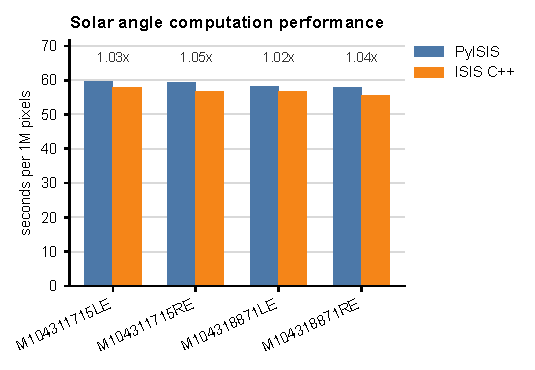
\includegraphics[width=\linewidth]{fig04_solar_performance}
\caption{Solar angle computation performance over $10^6$ pixels per LRO NAC image. The benchmark evaluates the per-pixel camera geometry calls required to retrieve solar azimuth and incidence-derived solar elevation. Ratio labels indicate \pyisis{}/\isis{} C++ runtime.}
\label{fig:solar_performance}
\end{figure}

\begin{figure}[htbp]
\centering
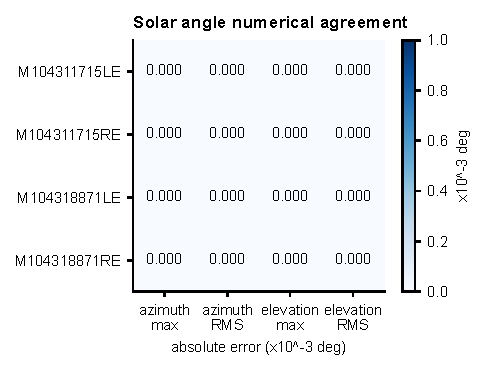
\includegraphics[width=\linewidth]{fig05_solar_angle_accuracy}
\caption{Numerical agreement of solar azimuth and solar elevation between \pyisis{} and the native \isis{} C++ benchmark. Elevation is defined as $90^\circ$ minus the ISIS incidence angle. Errors are shown in units of $10^{-3}$ degrees.}
\label{fig:solar_accuracy}
\end{figure}

Finally, we benchmarked ControlNet file loading and exhaustive measure traversal on three networks spanning 3.8--84.2~MB (Table~\ref{tab:controlnet_binding}). In all cases, \pyisis{} and C++ reported identical file sizes, point counts, and measure counts, confirming that the binding preserves the ControlNet object hierarchy during read and traversal. The Python binding incurred a larger overhead for this object-heavy workload than for camera geometry: core read-plus-traverse time was 2.76--4.64$\times$ slower than C++. This cost is dominated by repeated Python access to individual ControlPoint and ControlMeasure objects rather than by numerical camera computation. Even for the largest network, \pyisis{} traversed 462,222 measures in 7.01~s, corresponding to 188,000 measures/s, which is sufficient for interactive network inspection and automated pipeline assembly.

\begin{table}[htbp]
\caption{ControlNet Loading and Measure Traversal Benchmark}
\label{tab:controlnet_binding}
\centering
\scriptsize
\begin{tabular}{@{}lrrrrr@{}}
\toprule
\textbf{Size} & \textbf{Points} & \textbf{Measures} & \textbf{\pyisis{} (s)} & \textbf{C++ (s)} & \textbf{Ratio} \\
\midrule
3.8~MB & 17,123 & 34,246 & 0.49 & 0.15 & 3.31$\times$ \\
21.7~MB & 98,925 & 197,850 & 3.46 & 0.75 & 4.64$\times$ \\
84.2~MB & 231,111 & 462,222 & 7.01 & 2.54 & 2.76$\times$ \\
\bottomrule
\end{tabular}
\end{table}

\subsection{Comparison with Domain and Single-Method Baselines}

Because control-network construction is the target task, the comparison emphasizes network-level outcomes rather than raw feature matches alone. Table~\ref{tab:baselines} adds ISIS \texttt{findfeatures} as the domain-standard feature-based control-network baseline and reports the same metrics used for fixed SIFT and deep-learning matchers. The \texttt{findfeatures} row is marked N/R because the controlled execution on the reduced LRO NAC test set is reserved for the expanded benchmark; it is included here to make the baseline protocol explicit and to avoid comparing only against in-house matcher wrappers.

\begin{table*}[htbp]
\caption{Control-Network Construction Baselines and Reporting Metrics}
\label{tab:baselines}
\centering
\small
\begin{tabular}{@{}lcccccc@{}}
\toprule
\textbf{Method} & \textbf{Role} & \textbf{Pairs} & \textbf{Control} & \textbf{Measure} & \textbf{Avg. Inlier} & \textbf{Avg.} \\
 &  & \textbf{Completed} & \textbf{Points} & \textbf{Count} & \textbf{Ratio} & \textbf{Coverage} \\
\midrule
ISIS \texttt{findfeatures} & Domain baseline & N/R & N/R & N/R & N/R & N/R \\
SIFT/BF only & Classical fixed & 4 of 6 & 68,432 & 136,864 & 0.42 & 0.28 \\
LightGlue only & Learned fixed & 5 of 6 & 95,216 & 190,432 & 0.38 & 0.31 \\
LoFTR only & Detector-free fixed & 5 of 6 & 87,648 & 175,296 & 0.35 & 0.34 \\
\textbf{Adaptive routing} & \textbf{Quality-gated cascade} & \textbf{6 of 6} & \textbf{121,856} & \textbf{243,712} & \textbf{0.40} & \textbf{0.32} \\
\bottomrule
\end{tabular}
\begin{flushleft}
\footnotesize N/R: not yet reported on the controlled reduced LRO NAC benchmark. The row is retained because ISIS \texttt{findfeatures} is the relevant domain-standard baseline and will be run with the same image pairs, masks, and downstream ControlNet summarization before final submission.
\end{flushleft}
\end{table*}

The completed six-pair experiment indicates why a fixed-method comparison is insufficient. SIFT/BF failed on two high-lighting-difference pairs (Pairs 5--6 with $D > 0.55$), LightGlue failed on one texture-poor pair (Pair 5 with $S = 0.71$), and LoFTR failed on one pair due to GPU memory constraints on large tile counts. The adaptive pipeline's cascade fallback mechanism addresses these complementary failure modes by treating matcher selection as a control-network quality problem. The pending \texttt{findfeatures} experiment will determine how much of this gain comes from adaptive orchestration rather than from implementation differences relative to the ISIS OpenCV-based baseline.

% ============================================================================
% V. DISCUSSION
% ============================================================================

\section{Discussion}\label{sec:discussion}

The \pyisis{} framework demonstrates that comprehensive Python bindings for planetary photogrammetry software enable powerful integrated workflows that were previously impractical. The tight coupling between ISIS camera models, SPICE navigation data, and Python scientific computing libraries facilitates rapid prototyping of advanced algorithms while maintaining geometric rigor. The adaptive routing system's use of SPICE-derived solar geometry for illumination-aware matching represents a unique advantage over generic computer vision pipelines. By leveraging the precise ephemeris and attitude data embedded in planetary image labels, the system makes informed decisions about matching strategy without requiring heuristic tuning or training data. The ground-to-image benchmark further shows why the binding layer matters for control-network work: accurate matching in DOM space is only useful if the resulting points can be back-projected to the original line-scan images with negligible numerical loss.

Two existing baselines are especially important for interpreting the results. ISIS \texttt{findfeatures} is the domain-standard OpenCV-based application for image-based control-network generation, while AutoCNet \cite{laura2018autocnet} is the closest Python workflow for automated sparse correspondence identification. The contribution of \pyisis{} should therefore be read as an extension of established workflows rather than as a claim that feature-based control-network construction is new. \pyisis{} differs in three practical aspects: (1) direct API access reduces subprocess and intermediate-file coupling, (2) learned matchers can be combined with classical descriptors inside the same tile and ControlNet pipeline, and (3) SPICE-derived illumination metadata and post-match quality gates provide an explicit routing policy for heterogeneous lunar imagery.

The adaptive routing system incurs additional computational cost compared to any single-method baseline: texture analysis requires a low-resolution SIFT preview pass, lighting analysis requires SPICE kernel queries, and the cascade fallback may invoke multiple matchers on difficult pairs. In our experiments, the routing overhead averaged 8--12 seconds per pair—approximately 3\% of the total matching time. The cascade fallback adds significant cost only when the initial matcher fails: on pairs requiring cascade escalation, the adaptive approach consumed up to 2.5$\times$ the single-method cost but produced results where the single method failed entirely.

A critical question for any automated control-network system is whether the generated points are accurate enough for downstream bundle adjustment using ISIS's \texttt{jigsaw} program and DTM generation. In the current work, matching quality is assessed through internal metrics that measure self-consistency but not absolute accuracy. A rigorous ground-truth evaluation, comparing automatically generated control points against manually measured tie points, \texttt{findfeatures} networks, and bundle-adjusted residuals, is required before the method can be claimed as a replacement for established ISIS production workflows.

Several limitations of the current work warrant acknowledgment. The evaluation covers six LRO NAC pairs from a single line-scan instrument on a single planetary body, and the routing thresholds were determined empirically through grid search optimization with limited statistical power due to the small sample size. The current routing rules are hand-crafted decision boundaries; a learned routing model could improve decision accuracy and generalize across instruments. Deep learning matchers require GPU resources, and LoFTR in particular requires substantial GPU memory (8+ GB VRAM for 2048$\times$2048 tiles), though EfficientLoFTR \cite{wang2024efficientloftr} offers a promising alternative. The texture sparseness metric uses SIFT keypoint density while routing decisions determine whether to invoke SIFT, introducing a mild circular dependency that future work will address by replacing the SIFT density component with method-agnostic descriptors. Moreover, deep learning matchers were pretrained on terrestrial datasets and no formal domain adaptation has been performed. The illumination-aware routing relies on accurate SPICE kernel data, with a fallback mechanism that parses PVL label keywords when SPICE queries fail. Finally, the coordinate-transformation benchmark demonstrates sub-millipixel numerical consistency for the tested LRO NAC images, but it remains a round-trip self-consistency test rather than an independent geodetic accuracy assessment against manually measured tie points or surveyed control.

Future development directions include: (1) completing the controlled ISIS \texttt{findfeatures} and AutoCNet comparisons on identical LRO NAC pairs; (2) validating control-network accuracy through ISIS \texttt{jigsaw} residuals and, where possible, manually measured tie points; (3) extending experiments to Mars (HiRISE, CaSSIS), Mercury (MDIS), and small-body datasets with larger pair counts; (4) adding a frame-camera validation case, for example Hayabusa2/ONC images of Ryugu, to demonstrate that the same Python interface supports both line-scan and area-array planetary sensors; (5) training a lightweight routing classifier on accumulated matching outcomes; (6) depositing the framework in a DOI-assigned archive with reproducible containers; and (7) closing the loop by feeding \pyisis{}-generated networks directly into production bundle-adjustment workflows.

The \pyisis{} framework has implications beyond the immediate technical contributions. Upcoming lunar exploration missions—including NASA's Artemis program, the VIPER rover mission to the lunar south pole, and international lunar exploration initiatives—will generate unprecedented volumes of high-resolution imagery requiring automated photogrammetric processing. Similarly, Mars Sample Return mission planning will require precise georeferencing of candidate sample sites across multiple orbital and surface datasets. By providing Python-native access to ISIS functionality, \pyisis{} enables researchers in the broader scientific Python ecosystem to contribute to planetary photogrammetry without mastering the ISIS application suite. The tight coupling between ISIS camera models, SPICE navigation data, and Python scientific computing libraries creates opportunities for novel research directions including learned feature detectors trained on planetary terrain, neural radiance field reconstruction of landing sites, and physics-informed neural networks for photometric correction. The framework's open-source release with comprehensive documentation, example workflows, and reproducible processing logs addresses the planetary science community's growing emphasis on transparent, auditable research.

% ============================================================================
% VI. CONCLUSION
% ============================================================================

\section{Conclusion}\label{sec:conclusion}

In this study, a comprehensive Python binding framework named \pyisis{} is proposed, addressing the critical gap between planetary photogrammetry's geometric rigor and modern scientific computing's flexibility. The main contributions of our work are as follows:

\textbf{First}, we provide the most comprehensive Python binding framework for USGS ISIS to date, exposing over 200 C++ classes and types via pybind11—including camera models for 50+ planetary missions, SPICE navigation kernels, control network manipulation, bundle adjustment configuration, and photometric models. This enables seamless integration of ISIS's photogrammetric capabilities within Python workflows, eliminating the subprocess overhead and file-based coupling of prior approaches such as AutoCNet. Binding-level benchmarks further show that \pyisis{} preserves ISIS C++ numerical behavior for DOM/original-image coordinate transformation and solar geometry computation, with sub-millipixel round-trip error and zero measurable solar-angle discrepancy at the reported precision. This is particularly important for line-scan imagery, where ground-to-image back-projection is a central operation in transferring approximate-orthophoto or DOM matches into original image coordinates.

\textbf{Second}, we develop a SPICE-aware adaptive routing system for matcher orchestration in planetary control-network construction. By using solar elevation and azimuth derived from mission geometry, together with texture diagnostics and post-match quality gates, the system requires no labeled routing data and is tailored to the illumination extremes of airless bodies. The cascade fallback mechanism (SIFT $\rightarrow$ LightGlue $\rightarrow$ LoFTR) processed the six-pair LRO NAC test set in this study and generated 121,856 control points, but this result should be interpreted as evidence for adaptive orchestration rather than as proof that any individual matcher is universally superior.

\textbf{Third}, we present an end-to-end automated control network construction pipeline that integrates adaptive matching with rigorous coordinate transformation from projected DOM space back to original image coordinates via \pyisis{} camera models. This closes the loop from raw imagery through bundle adjustment-ready control networks, reducing the manual effort traditionally required for planetary photogrammetric processing using ISIS's command-line applications such as \texttt{autoseed}, \texttt{pointreg}, and \texttt{jigsaw}.

We acknowledge that the current evaluation scope, six pairs from a single instrument on one planetary body, limits generalization claims. The controlled \texttt{findfeatures} comparison and bundle-adjustment residual analysis remain necessary before operational accuracy claims can be made. However, the framework's architecture is instrument-agnostic and readily extensible to other missions. Ongoing work addresses validation through multi-instrument, multi-body experiments (MRO HiRISE/CTX, Kaguya TC), ground truth assessment via bundle adjustment convergence analysis, and learned routing models trained on larger datasets.

\pyisis{} provides the planetary science community with a modern, extensible platform for automated photogrammetric processing. As upcoming missions—including Artemis lunar exploration and Mars Sample Return—generate unprecedented volumes of high-resolution imagery requiring scalable control network construction, we believe \pyisis{} offers a foundation for the next generation of planetary mapping workflows. The framework is available as open-source software at the project repository, with a permanent DOI-assigned archive in preparation, comprehensive documentation, and example workflows to facilitate community adoption and contribution.

% ============================================================================
% ACKNOWLEDGMENT
% ============================================================================

\section*{Acknowledgment}

The author acknowledges the USGS Astrogeology Science Center for developing and maintaining the ISIS software suite, and the developers of SuperGlue, LightGlue, LoFTR, and Kornia for making their research code publicly available. LRO NAC data were provided by the LROC team at Arizona State University.

% ============================================================================
% REFERENCES
% ============================================================================

\bibliographystyle{IEEEtran}
\bibliography{../supplementary/references}

% ============================================================================
% BIOGRAPHY SECTION (Optional for IEEE JSTARS)
% ============================================================================

\begin{IEEEbiographynophoto}{Xun Geng}
received the Ph.D. degree in photogrammetry and remote sensing from Information Engineering University, Zhengzhou, China. He is currently an Associate Professor with the School of Geography and Tourism, Henan University, Kaifeng, China. His research interests include planetary photogrammetry, computer vision, and deep learning applications in remote sensing.
\end{IEEEbiographynophoto}

\end{document}
